\documentclass[a4paper, 11pt]{report}

%%%% Packages %%%%
\usepackage[utf8]{inputenc}
\usepackage[francais]{babel}
\usepackage{framed}
\usepackage{amssymb}
\usepackage{verbatim}
\usepackage{listings}
\usepackage[hidelinks]{hyperref}
\usepackage{float}

\usepackage[usenames,dvipsnames,table,xcdraw]{xcolor}
\usepackage[pdftex]{graphicx}
\usepackage{sectsty}
%% Couleurs
 \definecolor{orange}{HTML}{E74C3C}
 \definecolor{dark-blue}{HTML}{1A2530}
 \definecolor{blue}{HTML}{34495E}
 \definecolor{dkgreen}{rgb}{0,0.6,0}
 \definecolor{gray}{rgb}{0.5,0.5,0.5}
 \definecolor{mauve}{rgb}{0.58,0,0.82}
 
 \definecolor{part_color}{HTML}{E74C3C}
 \definecolor{section_color}{HTML}{2C3E50}
 \definecolor{subsection_color}{HTML}{34495E}
 
 \colorlet{shadecolor}{gray!7}

%% Parametres
\setcounter{tocdepth}{1}
\setlength{\parindent}{0pt}
\partfont{\color{part_color}}
\sectionfont{\color{section_color}}
\subsectionfont{\color{subsection_color}}
\makeatletter
\@addtoreset{section}{part}
\makeatother  


%% Commandes
\renewcommand{\thesection}{\Roman{section}}
\renewcommand{\thesubsection}{\arabic{subsection}} % Les sections n'affichent pas le numero du chapitre
\newcommand{\includecode}[1]{\lstinputlisting{#1}}

\newcommand{\HRule}{\rule{\linewidth}{0.5mm}}
%% Environements
\renewenvironment{shaded}
	{
  	\def\FrameCommand{\fboxsep=\FrameSep \colorbox{shadecolor}
  	}
  	\MakeFramed{\advance\hsize-\width \FrameRestore\FrameRestore}}
 {\endMakeFramed}
 
 \lstset{frame=tb,
  language=Java,
  aboveskip=3mm,
  belowskip=3mm,
  showstringspaces=false,
  columns=flexible,
  basicstyle={\scriptsize\ttfamily},
  numberstyle=\tiny\color{gray},
  keywordstyle=\color{blue},
  commentstyle=\color{dkgreen},
  stringstyle=\color{mauve},
  tabsize=2,
}

\lstset{literate=
  {á}{{\'a}}1 {é}{{\'e}}1 {í}{{\'i}}1 {ó}{{\'o}}1 {ú}{{\'u}}1
  {Á}{{\'A}}1 {É}{{\'E}}1 {Í}{{\'I}}1 {Ó}{{\'O}}1 {Ú}{{\'U}}1
  {à}{{\`a}}1 {è}{{\`e}}1 {ì}{{\`i}}1 {ò}{{\`o}}1 {ù}{{\`u}}1
  {À}{{\`A}}1 {È}{{\'E}}1 {Ì}{{\`I}}1 {Ò}{{\`O}}1 {Ù}{{\`U}}1
  {ä}{{\"a}}1 {ë}{{\"e}}1 {ï}{{\"i}}1 {ö}{{\"o}}1 {ü}{{\"u}}1
  {Ä}{{\"A}}1 {Ë}{{\"E}}1 {Ï}{{\"I}}1 {Ö}{{\"O}}1 {Ü}{{\"U}}1
  {â}{{\^a}}1 {ê}{{\^e}}1 {î}{{\^i}}1 {ô}{{\^o}}1 {û}{{\^u}}1
  {Â}{{\^A}}1 {Ê}{{\^E}}1 {Î}{{\^I}}1 {Ô}{{\^O}}1 {Û}{{\^U}}1
  {œ}{{\oe}}1 {Œ}{{\OE}}1 {æ}{{\ae}}1 {Æ}{{\AE}}1 {ß}{{\ss}}1
  {ç}{{\c c}}1 {Ç}{{\c C}}1 {ø}{{\o}}1 {å}{{\r a}}1 {Å}{{\r A}}1
  {€}{{\EUR}}1 {£}{{\pounds}}1
}

    
\newenvironment{vulgarisation}
    {
    \textit{\textcolor{dark-blue}{$\blacksquare$  Vulgarisation : \\}}

    }
    {
    ~\\\textcolor{dark-blue}{$\blacksquare$}\\
    }
    
\newenvironment{formalisation}
    {
    \textit{\textcolor{blue}{$\blacksquare$  Formalisation : \\}}
    }
    {
    ~\\\textcolor{blue}{$\blacksquare$}\\
    }
    
\newenvironment{codage}
    {
    \textit{\textcolor{gray}{$\blacksquare$  Règle JAPE : \\}}
    }
    {
    ~\\\textcolor{gray}{$\blacksquare$}\\
    }
    
\newenvironment{exemple}
    {
    \textit{\textcolor{orange}{
    Exemple : \\}}
    }
    {~\\
    }

\begin{document}

%% Couverture
\author{Charles Follet \and Roland Bary}

\begin{titlepage}
\begin{center}

% Upper part of the page. The '~' is needed because \\
% only works if a paragraph has started.

\includegraphics[width=0.25\textwidth]{./logo.png}~\\[1cm]

\textsc{\Large Projet Tutoré}\\[0.5cm]
\textsc{\Large M1 Technologies de l'Internet}\\[0.5cm]

% Title
\HRule \\[0.4cm]
{ \LARGE \bfseries Conception et développement d’une application d’annotation thématique dans
l'environnement Gate \\[0.4cm] }

\HRule \\[1.5cm]

% Author and supervisor
\noindent
\begin{minipage}[t]{0.4\textwidth}
\begin{flushleft} \large
\emph{Auteurs:}\\
Roland \textsc{Bary}\\
Charles \textsc{Follet}
\end{flushleft}
\end{minipage}%
\begin{minipage}[t]{0.4\textwidth}
\begin{flushright} \large
\emph{Tuteurs:} \\
Marie-Noëlle \textsc{Bessagnet}\\
Annig \textsc{Lacayrelle}\\
Albert \textsc{Royer}\\
Christian \textsc{Sallaberry}
\end{flushright}
\end{minipage}

\vfill

% Bottom of the page
{\large \date{}}

\end{center}
\end{titlepage}
\section*{Remerciements}
Nous tenons à remercier nos tuteurs pour leur pédagogie et leur encadrement. Monsieur Royer pour sa précision et sa connaissance pointue du domaine. Madame Lacayrelle pour son soutien et sa clarté. Monsieur Sallaberry pour nous avoir remis sur de bonnes pistes quand nous nous égarions. Et enfin, madame Bessagnet pour avoir assuré la coordination et le suivi de ce projet.
\tableofcontents

\part{Introduction}
L'évolution des volumes d'informations sur internet provoque une évolution du web vers une approche dans laquelle chaque donnée acquiert un sens afin de rendre possible une interprétation du contenu par des machines. Cette évolution constitue le web sémantique.\\
Sa principale motivation  est la recherche d’information sémantique.\\

Dans ce cadre, nous sommes intervenus pour répondre à l'appel d'offre de la maîtrise d'ouvrage. \\
L'objectif correspond à la première étape dans un processus de recherche d'information sémantique et d'indexation : l'annotation sémantique d'un document texte spécifique.\\

En découle les problématiques suivantes :
\begin{itemize}
\item Existe-t-il des outils qui se prêtent aisément à l'annotation sémantique ?
\item Quelle approche de conception nous permet de réaliser cette étape d'annotation sur un document texte non-structuré ?
\end{itemize}
	~\\
	
La résolution de ces différentes problématiques nous a amenés à organiser notre réflexion :\\
Premièrement, nous définirons clairement les demandes et leurs contextes à travers le cahier des charges. Deuxièmement, nous présenterons les connaissances qu'il nous a fallu maîtriser pour ce sujet. Troisièmement, nous détaillerons notre principe de résolution du projet. Nous finirons par le bilan et le retour d’expérience de ce projet.
\part{Cahier des charges}
	\section{Contexte}

A partir des travaux de Georges DEPEYROT sur les monnaies carolingiennes, nous avons travaillé sur l'annotation du Numéraire Carolingien\footnote{\url{http://www.cgb.fr/le-numeraire-carolingien-moneta-77-3e-edition-depeyrot-georges,Ln71,a.html}}.\\
Sur celui-ci, la maîtrise d'ouvrage a besoin d'effectuer des recherches :

\begin{description}
\item [Temporelles] : Quelles étaient les pièces en circulation de l'an 859 à l'an 865?
\item [Spatiales] : Dans quels ateliers, les pièces de type Obole de Charlemagne ont été produites ? 
\item [Thématiques] : Combien d'exemplaires de la monnaie d'or de Charles le Chauve ont été étudiés ?
\end{description}

Répondre à cette demande implique de définir puis d'explorer les dimensions temporelles, spatiales et thématiques de l'ouvrage.\\
Pour cela, il est nécessaire de connaître le domaine et l'ouvrage afin de savoir quelle information correspond à quelle dimension.\\
Une fois cet apprentissage fait, nous pouvons construire des règles dans une chaîne de traitement permettant d'annoter chaque information en fonction de sa dimension. \\

Les monnaies carolingiennes sont le domaine central pour la réalisation du projet. Les ressources nécessaires à l'annotation (ici sous forme de gazetiers) ont été construites à partir des données de l'ouvrage.\\

Forte de son expérience dans le domaine, la maîtrise d'ouvrage nous a demandé d'utiliser la boîte à outils logicielle GATE qui sera utile pour le traitement du langage naturel.\\~\\

En résumé, les caractéristiques du projet sont : 
\begin{itemize}
\item l'apprentissage et la compréhension du domaine considéré,
\item l'étude des principes d'annotation de documents,
\item le développement d'une chaîne d'annotation dans GATE,
\item la mise en place d'une visualisation des résultats.
\end{itemize}

\newpage
	\section{Description}
	La chaîne de traitement prend un document texte en entrée, produit un document XML en sortie et le met en forme pour une meilleure lisibilité.\\
	\begin{exemple}
\noindent Illustrons par un scénario les objectifs de la chaîne de traitement.
Elle prend par exemple en entrée le texte suivant

\begin{figure}[h!]
\centering
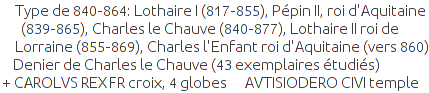
\includegraphics[scale=.5]{img/exemple_text.png}
\end{figure}

et l'annote
\end{exemple}
\begin{figure}[h!]
\centering
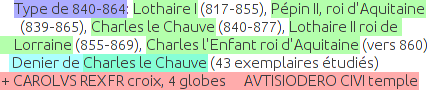
\includegraphics[scale=.5]{img/exemple_text_ann.png} 
\end{figure}\\
Chaque information pertinente est annotée. En bleu la période d'émission de la monnaie (Temporel), en vert les souverains qui l'ont faite produire (Thématique), en cyan la nature de la monnaie (Thématique) et en rouge la légende (Thématique).\\
Afin de développer cette chaîne,nous avons dû planifier notre travail et nos réunions avec la maîtrise d'ouvrage. Cette planification sera présentée dans la partie suivante.

	\section{Diagramme de Gantt prévisionnel}
	\begin{figure}[H]
	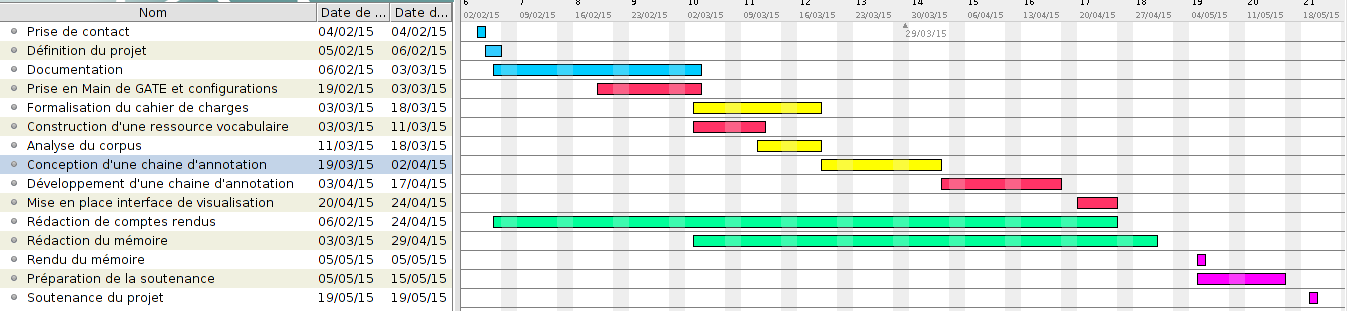
\includegraphics[scale=.3]{img/ganttPrev.png}
	\end{figure}
	Dans ce planning, nous avions prévu une première phase de documentation sur les différents concepts et technologies que nous allions utiliser. \\
En parallèle, nous devions nous mettre d’accord avec les responsables du projet sur le travail à effectuer, grâce au cahier des charges.
Ensuite, nous avions la phase de développement durant laquelle nous allions mettre en place notre chaîne de traitement et notre interface de visualisation. Tout au long du projet nous devions rédiger les différents comptes rendus de réunion et le mémoire.\\
Évidemment, ce diagramme ne représente en aucun cas la façon dont s’est réellement déroulé notre projet.
\part{Cadre d'analyse}
\section*{Introduction}
Pour cerner l'environnement du projet, nous allons définir quelques connaissances liées au domaine de l'annotation sémantique. Ensuite, viendra une description des outils qui ont été nécessaires lors de la phase de développement.\\

\section{Définition de concepts}
L'annotation sémantique peut se définir comme une activité qui va mettre une "note" sur une partie d'un texte. Elle permet de travailler plus facilement sur un texte en apportant une sur-couche d'informations, qui va donner un sens aux textes.\cite{GLNS09}
\subsection{Le web sémantique}
Le Web sémantique, ou toile sémantique, est un mouvement collaboratif mené par le World Wide Web Consortium (W3C) qui met en place des méthodes communes pour échanger des données.\\
Il favorise l'émergence de nouvelles connaissances en s'appuyant sur celles déjà présentes sur Internet en les structurant et en les liant.\\
Selon le W3C, ``le Web sémantique fournit un Modèle qui permet aux données d'être partagées et réutilisées entre plusieurs applications, entreprises et groupes d'utilisateurs''.\\
L'expression a été inventée par Tim Berners-Lee, inventeur du World Wide Web et directeur du World Wide Web Consortium qui supervise le développement des technologies communes du Web sémantique.\\
Le directeur du W3C définit le Web sémantique comme ``un web des données qui peuvent être traitées directement et indirectement par des machines pour aider leurs utilisateurs à créer de nouvelles connaissances''. \cite{w1ws}

\subsection{Les entités nommées}
Les entités nommées sont des objets textuels (mot, ou groupe de mots) catégorisés dans des classes. Celles-ci peuvent être les noms de personnes, noms d'organisations, noms de lieux, quantités, distances, dates, auxquelles on associe un identifiant unique.\cite{w2re}\\
Les entités nommées sont "associées à des expressions linguistiques sollicitées par des applications qui manipulent des documents textuels".p33 \cite{DN12}\\
Voici l'illustration d'une recherche d'entités nommées :
\begin{verbatim}
Henri a acheté 300 actions de la société AMD en 2006
<ENAMEX TYPE="PERSON">Henri</ENAMEX> a acheté 
<NUMEX TYPE="QUANTITY">300</NUMEX> actions de la société 
<ENAMEX TYPE="ORGANIZATION">AMD</ENAMEX> en 
<TIMEX TYPE="DATE">2006</TIMEX>.
\end{verbatim}
La reconnaissance et la résolution d'entités nommées peut s'avérer difficile dans la mesure où elles sont sujettes à des ambiguïtés liées aux phénomènes linguistiques tel que: la synonymie, l'homonymie ou encore la métonymie. p44\cite{DN12}\\
\begin{exemple}
Avec l’entité nommée "Paris" au sein des énoncés suivants:
\begin{itemize}
\item "La star \textbf{Paris} Hilton s'est achetée un nouveau chien." (Personne)
\item "Je suis parti en vacances à \textbf{Paris}." (Lieu)
\item "Le \textbf{Paris} Saint-Germain a battu Marseille à domicile." (Organisation sportive)
\end{itemize}
\end{exemple}

\subsection{Les gazetiers}
Un gazetier peut être assimilé à un ensemble de listes contenant des noms d'entités. Elles peuvent être des villes, des organisations, des jours de la semaine, des métiers, etc. Ces listes sont utilisées pour trouver des occurrences de ces noms dans un texte, comme pour l'activité de recherche d'entités nommées.\\
Le terme Gazetier est souvent utilisé de manière interchangeable pour un ensemble de listes d'entités et de ressources permettant de trouver des occurrences de noms dans un texte.\\
Chaque gazetier est fichier texte d'extension "lst" avec une entrée par ligne.\cite{w4gaz}
Ci-dessous un exemple de Gazetier:
\begin{figure}[H]
\begin{center}
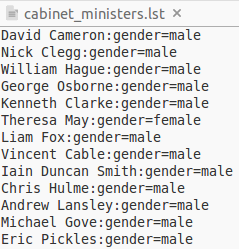
\includegraphics[scale=0.5]{img/exGazetier.png}
\end{center}
\caption{Exemple de Gazetier}
\end{figure}
Sur chaque ligne, on distingue plusieurs colonnes de par des séparateurs (\textbf{:} , \textbf{;} , ...). La première colonne correspond à la valeur d'une entité, la seconde constitue le MajorType (Type principal d'annotation) de l'entité et la troisième le MinorType (Type secondaire d'annotation).\cite{w4gaz}
\subsection{Les expressions régulières}
Les expressions régulières sont une famille de notations compactes et puissantes pour décrire certains ensembles de chaînes de caractères. Elles permettent de rechercher automatiquement des morceaux de texte ayant certaines formes, et éventuellement remplacer ces morceaux par d'autres.
Les expressions régulières sont utilisées par un grand nombre d'éditeurs de textes et utilitaires (particulièrement sous Unix), par exemple Vim, Emacs, sed ou awk. On les retrouve également dans la majorité des langages de programmation modernes.\cite{w3}\
Exemple d'utilisation d'une expression régulière sur un bout de texte:
\begin{itemize}
\item Expression : \verb|(?:\d*\.)?\d+|
\item Texte: \textbf{10}rats + \textbf{.36}geese = \textbf{3.14}cows
\end{itemize}
\section{Outils}%%%%%%%%%%%%%%%%%%%%%%%%%%%%%%%%%%%%%%%%%%%%%%%%%%%%%%%%%%%%%%%%%%%%
(Il est indiqué dans notre cahier de charge, que l'annotation des textes, devra se faire dans l'environnement GATE. Il est donc impératif pour nous, de présenter cet outil.)
\subsection{L'environnement GATE}
GATE est un logiciel développé en Java à l’université de Sheffield en 1995 et utilisé pour
le traitement du langage naturel, y compris l’extraction d’information dans de nombreuses
langues. 
\subsubsection{Fonctionnement général}
C'est un outil qui repose sur le principe d'une chaîne de traitement ("pipeline") constituée de plusieurs modules (dits "Processing ressources" PR) appliqués successivement sur un ou plusieurs textes (dits "Languages Ressources" LR). Les documents donnés en entrée peuvent être un simple texte ou un corpus en local (cf. figure 2), que l'on charge avec une URL. Les différents composants annotent chacun à leur tour le texte en prenant en compte les annotations précédentes puis le document est retourné à l'utilisateur au format XML. pp19-20\cite{SL10}
\begin{figure}[H]
\begin{center}
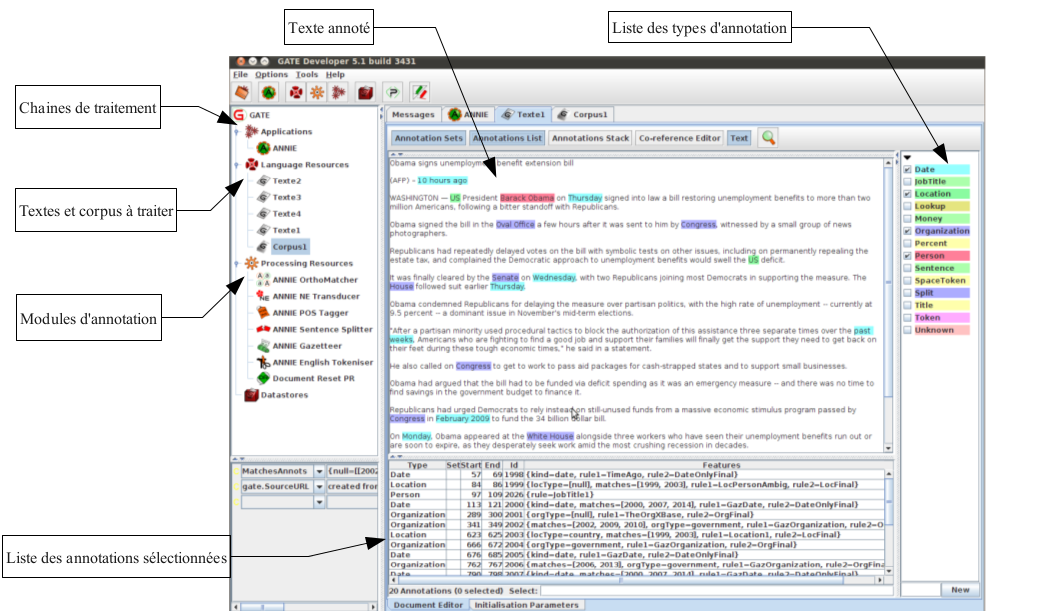
\includegraphics[scale=0.3]{img/exempleAnnotationGATE.png} 
\end{center}
\caption{Exemple de texte annoté dans l'outil GATE}
\end{figure}
Par un système de plugins, GATE met à disposition de ses utilisateurs un grand nombre de
modules dédiés à l'analyse textuelle. Les plus courants sont les segmenteurs (Tokenizers), les
étiqueteurs morpho-syntaxiques (Part Of Speech Taggers), les lexiques (Gazetteers) ou encore les
transducteurs (JAPE transducers). L'interface graphique permet de charger de nouveaux plugins et
ressources, de les paramétrer et de les combiner au sein d'une même chaîne de traitement (cf.figure 3). p22\cite{SL10}
\begin{figure}[H]
\begin{center}
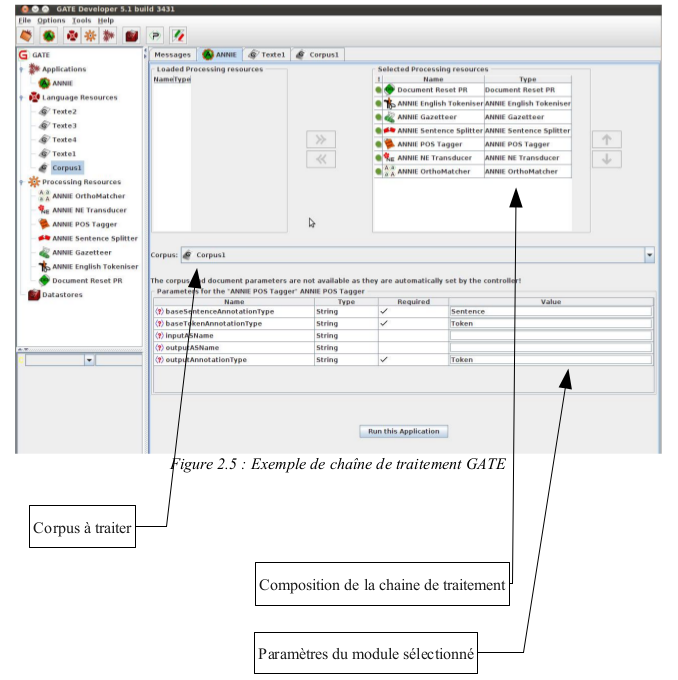
\includegraphics[scale=0.3]{img/exempleChaineTraitement.png}
\end{center}
\caption{Processus d'annotation}
\end{figure}
GATE comprend entre autres un système d'extraction d'information nommé ANNIE. Il est constitué d'un certains nombre de modules, y compris ceux énoncés dans le paragraphe précédent. ANNIE est une chaîne de traitement par défaut et peut servir de point de départ pour des tâches plus spécifiques.
\subsubsection{La chaîne de traitement ANNIE}
\begin{figure}[H]
\begin{center}
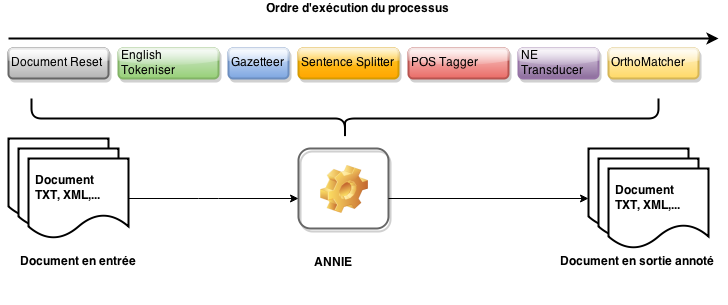
\includegraphics[scale=0.5]{img/annieChaine.png} 
\end{center}
\caption{Représentation de la chaîne de traitement ANNIE}
\end{figure}
\begin{description}
\item[Document Reset] nettoie toutes les annotations précédentes et remet le
corpus de documents à son état initial.
\item[Tokeniser] divise le texte en annotation de type Token comme par exemple les chiffres, les
signes de ponctuation et des mots.
\item[Gazetteer] identifie les noms des entités qui se trouvent dans le texte, sur la base d’un gazetier.
\item[Sentence Splitter] applique une multitude de transducer à états finis qui segmente le texte en
phrases.
\item[POS Tagger] attribue une catégorie linguistique à un token (Ex: NNP pour les noms propres au singulier).
\item[NE Transducer] tente de trouver les entités nommées inconnus en fonction de modèles d'extraction écrits dans le langage JAPE (expliqué dans la sous-partie suivante).
\item[OrthoMatcher] ajoute une relations d'identité entre les entités nommées trouvées par le NE Transducer, afin d'effectuer une coréférence. p24 \cite{SL10}
\end{description}
\subsection{Le formalisme JAPE}
Une partie des différents modules proposés dans GATE est basé sur le formalise JAPE (Java Annotation Patterns Engine), un transduceur à états finis permettant de reconnaître des expressions régulières sur les annotations. Ce système s'avère très utile en extraction d'informations car il permet de définir les contextes d'apparition des éléments à extraire pour ensuite les repérer et les annoter. Le principe consiste à combiner différentes annotations dites basiques (tokens, relations syntaxiques, etc) pour en créer de nouvelles plus complexes (entités nommées, relations, événements, etc.). Cela revient à l'écriture de règles de production et donc à l'élaboration d'une grammaire régulière.\\
Une grammaire JAPE se décompose en plusieurs phases exécutées consécutivement et formant une cascade d'automates à états finis. Chaque phase correspond à un fichier « .jape » et peut être constituée d'une ou plusieurs règle(s) écrite(s) selon le formalisme associé à JAPE. p23\cite{SL10}\\
Classiquement, ces règles sont divisées en deux blocs : 
\begin{itemize}
\item une partie gauche (« Left Hand Side » ou LHS) définissant un motif d'annotations à repérer,
\item une partie droite (« Right Hand Side » ou RHS) contenant les opérations à effectuer sur ce motif.
\end{itemize}
Le lien entre ces deux parties se fait par l'attribution d'une étiquette au motif (ou à ses constituants) en LHS et par sa réutilisation en RHS pour y appliquer les opérations nécessaires.\cite{SL10}\\
Pour plus de clarté, prenons l'exemple d'une règle simple :\\
\begin{exemple}
\begin{verbatim}
1.	Rule: OrgAccronym
2.	((
3.		{Organisation}
4.		{Token.string == "("}
5.		({Token.orth == "allCaps"}):org
6.		{Token.string == ")"}
7.	 )
8.	 -->
9.	:org.Organisation = {rule = "OrgAcronym"}
\end{verbatim}

L'objectif de cette règle est d'annoter en tant qu'organisation les acronymes entre parenthèses positionnés après une annotation de type "Organisation". Tout d'abord, l'on commence par donner un nom à la règle (l1). Les lignes 2 à 7 définissent le motif à repérer dans le texte. Le signe \verb|-->| (ligne 8) sert de séparateur entre LHS et RHS. Enfin, la dernière ligne (ligne 9) exprime l'opération souhaitée.
\end{exemple}

Précisons quelques règles syntaxiques de base du formalisme JAPE:
\begin{itemize}
	\item La partie gauche de la règle est toujours entre parenthèses
	\item La partie droite commence par le signe \verb|"-->"|
	\item Les types d'annotation sont encadrés par des accolades
	\item \verb|"Token.string"| permet d'obtenir la valeur de la propriété \verb|"string"| associé à l'annotation \verb|"Token"|
	\item \verb|":org"| permet d'identifier une partie du motif en LHS pour l'utiliser en RHS
	\item La ligne 9 attribue une annotation de type "Organisation" au segment étiqueté "org" en LHS; l'ajout de la propriété "rule" à cette annotation permet d'indiquer quelle règle en est à l'origine.
\end{itemize}
La liste des annotations utilisées en LHS de la règle est déclarée en début de phase grâce à l'attribut « Input » : par exemple, « Input : Lookup, Token, Person ». Par ailleurs, l'attribut « Control » permet de définir l'ordre d'exécution des différentes règles d'une phase et « Debug »
d'obtenir un affichage des éventuels conflits rencontrés entre règles.
Pour finir, précisons qu'un système de macros est également disponible : une macro permet
de définir et de nommer une séquence d'annotations afin de la réutiliser plus rapidement par la suite. p23 \cite{SL10}\\
Ci-dessous un exemple de règle JAPE plus complet incluant l'utilisation des macros:\\
\begin{exemple}
\begin{verbatim}
Phase: pourcent
Input: Lookup Token
Options: control = appelt
Macro: AMOUNT_NUMBER
(
	({Token.kind == number}
	(
		({Token.string == ","} | {Token.string == "."})
		{Token.kind == number}
	)?
	(
		{Token.string == "-"}
		{Token.kind == number}
	)?
	)
)
Macro: PERCENT
(
	{Token.string == "%"} |
	{Token.string == "pourcent"}|
	({Token.string == "pour"}{Token.string == "cent"})
)
Macro: LIAISON_PERCENT_DE_ET
(
	{Token.string == "de"}|
	{Token.string == "et"}|
	{Token.string == ","}
)
Rule: Percent_number
(
	((AMOUNT_NUMBER)
	({Token.string == "à"})
)?
	(AMOUNT_NUMBER)
	(PERCENT)
)
:pourcent -->
:pourcent.Percent = {Kind="pourcent",Rule="Percent_number"}
\end{verbatim}
\end{exemple}
Pour formuler une règle JAPE, il est utile de connaître le formalisme des expressions régulières présentées en amont. Il est également utile de pouvoir tester et vérifier syntaxiquement et sémantiquement les expressions régulières réalisées.
\newpage
\subsection{RegExr : Outil en ligne pour manipuler des expressions régulières}
RegExr\footnote{http://www.regexr.com/} est un outil de manipulation d’expressions régulières écrit en Javascript.
Les avantages de cet outil sont : 
\begin{itemize}
\item la coloration syntaxique,
\item la visualisation temps réel du résultat dans un texte personnalisable,
\item l'aide appropriée
\item une communauté partageant ses expressions régulières
\end{itemize}
\begin{figure}[h]
\begin{center}
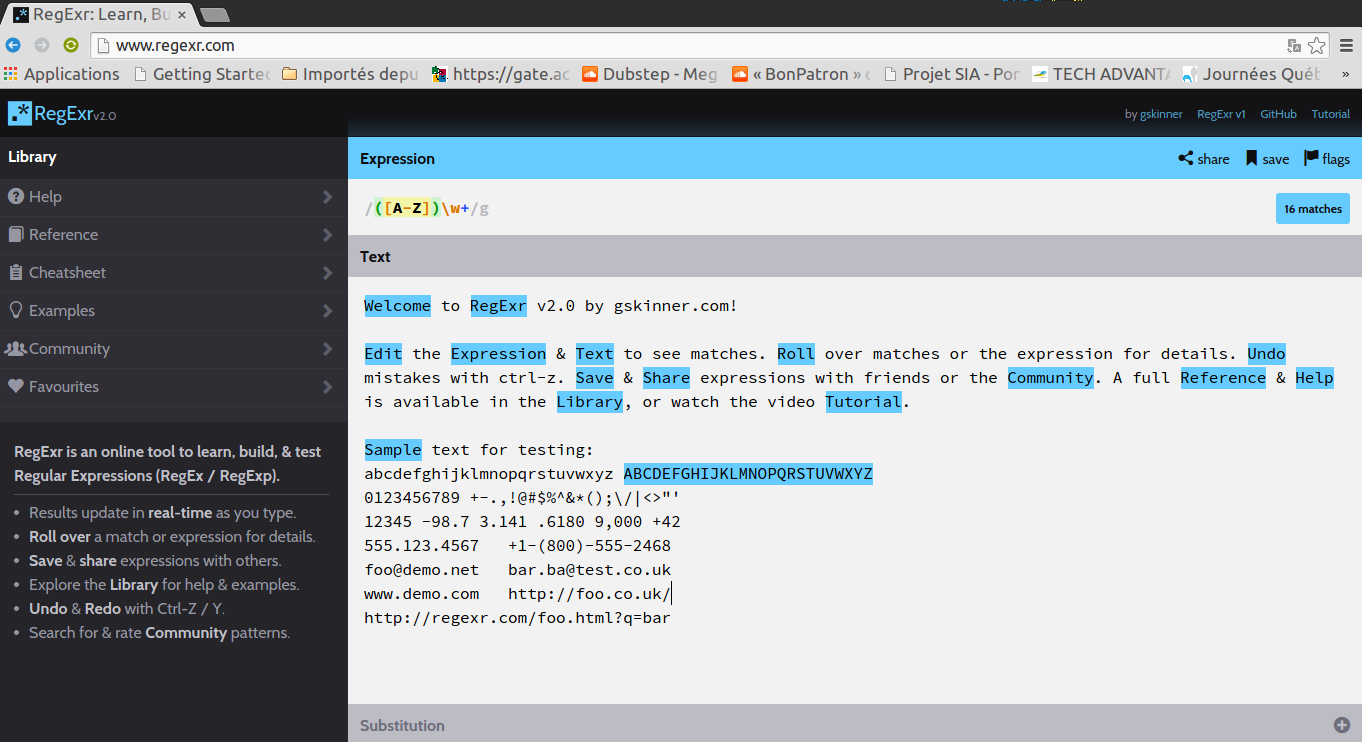
\includegraphics[scale=0.3]{img/regexr.png} 
\end{center}
\caption{Exemple de manipulation d'expression régulière dans RegExr}
\end{figure}
\part{Développement}
	\section*{Introduction}
	Avant de démarrer le développement de la chaîne de traitement, nous devons nous familiariser avec notre environnement de travail. Ensuite, nous allons pouvoir définir nos annotations, leur domaine et choisir de quelle façon nous allons les capturer.
	\section{Prise en main de l'environnement}
	Au lancement du projet, la seule ressource à disposition était le Numéraire Carolingien au format papier. Il fallait le numériser et l'OCRiser\footnote{Reconnaissance optique de caractères}.\\
    Nous avons numérisé une cinquantaine de pages à la main pour les OCRiser automatiquement par la suite à l'aide de l'outil \texttt{tesseract}.\\

    L'OCRisation s'est déroulée de la façon suivante : 
    \begin{figure}[h]
    \centering
    
\includegraphics[scale=.3]{img/OCRisation.png}
    \end{figure}\\
    La scanner que nous avons utilisé permettait d'obtenir une image pour chacune des pages au format PDF. Ensuite, étant donné que  \texttt{tesseract} est plus performant et précis avec des fichiers TIFF, il a fallu convertir les fichiers PDF en TIFF. Cependant, quelques erreurs d'OCRisation sont apparues. Pour finir,  \texttt{tesseract} nous donnait des fichiers TXT.\\
    Les étapes de conversion du schéma précédent ont été réalisées à l'aide de script en langage SHELL:
    \begin{enumerate}
        \item \begin{enumerate}
    	      \item	
           \begin{verbatim}
for file in *.pdf
do
  convert -density 300 ../pdf/$file
          -depth 8 `basename $file .pdf`.tiff
done
           \end{verbatim}
          \item les pages impaires ont été numérisées à l'envers, il fallait les mettre dans le bon sens.
          \begin{verbatim}
for file in *.tiff
do
    if [ $((`basename $file .tiff` % 2 )) = 1 ]; then
        convert $file -rotate 180 $file;
    fi
done
          \end{verbatim}
       \end{enumerate}
    \item 
    \begin{verbatim}
for file in img/*.tiff
do
  tesseract $file txt/`basename $file .tiff` -l fra
done 
    \end{verbatim}
    \end{enumerate}
    
	\section{Définition des dimensions d'annotation et leur contenu}
    Dans l'introduction, nous avons vu qu'il y a trois dimensions d'annotation mais ne les avons pas définies.\\
	\textit{Note : Le détail de chaque annotation peut être trouvé dans les parties III et IV.}
    \subsection{Dimension spatiale}
    \subsubsection{Définition}
     La dimension spatiale contient toutes les informations de lieux. Peu spécifique au domaine considéré.
    \subsubsection{Contenu}
       Le contenu de cette dimension est minime. Hormis les ateliers appartenant à la dimension thématique, les lieux présents dans le document n'intéressent que très peu la maîtrise d'ouvrage. Nous n'avons donc pas de contenu pour cette dimension.
	\subsection{Dimension temporelle}
	    \subsubsection{Définition}
    La dimension temporelle contient toutes les informations de temps et de durées. Peu spécifique au domaine considéré.\\
    \subsubsection{Contenu}
    \begin{description}
    \item[les périodes d'émission] des monnaies,
    \item[les périodes de règne] des souverains.
    \end{description}
    
	\subsection{Dimension thématique}
	    \subsubsection{Définition}
    La dimension thématique contient toutes les informations spécifiques au domaine considéré.  C'est à dire les informations propres aux monnaies carolingiennes.
    \subsubsection{Contenu}	
    \begin{description}
    \item[La nature] des monnaies,
    \item[La légende] des monnaies
    \item[Le type] des monnaies,
    \item[Les collections] des monnaies,
    \item[Les trésors] des monnaies,
    \item[Les trouvailles] des monnaies.
    \end{description}
    
    
	\section{Première recherche d'entités nommées avec les gazetiers}
	\subsubsection{Ateliers}
\begin{vulgarisation}
	L'ouvrage est décomposé en ateliers qui donnent leur nom à chaque début de "partie" ou "chapitre". Ce nom correspond à un endroit de France ou pays limitrophes dans lequel est produite la monnaie. Ce lieu peut être une ville, un lieu-dit dont le nom peut ne plus exister. Il fût donc difficile de trouver un pattern via les expressions régulières. Nous avons alors dû construire ce gazetier à partir de la liste en début d'ouvrage qui recense tous les ateliers.
\end{vulgarisation}
\begin{formalisation}
\begin{verbatim}
Aix-la-Chapelle (Allemagne)
Agen (Lot-et-Garonne)
Aix-la-Chapelle
Alsheim (Allemagne)
Altenheim (Bas-Rhin)
Amiens (Somme)
\end{verbatim}
\end{formalisation}

\subsubsection{Souverains}
\begin{vulgarisation}
	Les nom des souverains ont des formats aussi divers que variés. Ils comportent des majuscules, des chiffres romains... Il serait difficile d'utiliser une expression régulière pour espérer annoter cette information. Il est plus judicieux d'utiliser un gazetier. Il sera construit à partir du début du numéraire. 
\end{vulgarisation}
\begin{formalisation}
\begin{verbatim}
Pépin le Bref:valeur=Pépin le Bref:periode=752-768
Adalbert Lothaire:valeur=Adalbert Lothaire:periode=954-986
Amoul roi de Germanie:valeur=Amoul roi de Germanie:periode=887-899
Bérenger I:valeur=Bérenger I:periode=888-924
Bérenger II:valeur=Bérenger II:periode=950-961
\end{verbatim}
\end{formalisation}

	\section{Deuxième recherche d'entités nommées avec les règles JAPE}
	\subsubsection{Périodes}
\begin{vulgarisation}
	\textit{Période} : intervalle de deux dates séparées par un tiret.\\
	\begin{exemple}
		\textit{757/8-786}
	\end{exemple}
	
	Une période est un intervalle entre deux dates. Dans notre travail, les dates sont constituées de trois et seulement trois chiffres. En cas d'ambiguïté, chacune d'entre elles peut être suivie d'un \og/\fg{} et d'un chiffre traduisant l'indétermination de la date.\\
	\begin{exemple}
		\textit{757/8}
	\end{exemple}
	
\end{vulgarisation}
\begin{formalisation}
	\textit{Date}
	\begin{verbatim}
([0-9]{3}\/?[0-9]?)
	\end{verbatim}
	\textit{Période}
	\begin{verbatim}
([0-9]{3}(\/[0-9])?)-([0-9]{3}(\/[0-9])?)
	\end{verbatim}
	\begin{exemple}
		"\emph{Type de 771-793/4: Charlemagne (768-814),...}" \\
		Group \#1 : 771 \\
		Group \#2 : 793/4\\\\\noindent
		Group \#1 : 768 \\
		Group \#2 : 814
	\end{exemple}
\end{formalisation}
	\begin{codage}
	\begin{lstlisting}
		// Regle JAPE
	Macro: TROIS_NOMBRES
({Token.kind==number,Token.length == 3})

Macro: UN_NOMBRE
({Token.kind==number,Token.length == 1})

Macro:SLASH
({Token.string=="/"})

Macro:DATE_PRECISE
(TROIS_NOMBRES)

Macro:DATE_IMPRECISE
(TROIS_NOMBRES SLASH UN_NOMBRE)

Macro:DATE
(DATE_PRECISE | DATE_IMPRECISE)

Rule: PeriodeRule
(
	(DATE):d1({Token.string =="-"})(DATE):d2
    ):Periode -->
:Periode{/*Code java pour extraire les extremites de l'intervalle*/}
	\end{lstlisting}
	\end{codage}
	
\newpage
\subsubsection{Périodes d'émission}
\begin{vulgarisation}
	Une période d'émission a la forme suivante :  \og Type de \{Période\} : \fg{} (Période étant l'annotation définie précédemment).\\
	Il faut sécuriser la capture de la période d'émission en ajoutant la contrainte précédée de "Type de" afin de ne pas récupérer toutes les périodes du document.
\end{vulgarisation}
\begin{formalisation}
	\begin{verbatim}
Type de : ([0-9]{3}(\/[0-9])?)-([0-9]{3}(\/[0-9])?)
	\end{verbatim}
	\begin{exemple}
		"\emph{Type de 771-793/4: Charlemagne (768-814)...}" \\
		Group \#1 : 771 \\
		Group \#2 : 793/4
	\end{exemple}

\end{formalisation}
			\begin{codage}
	\begin{lstlisting}
	// Regle JAPE
	Macro: CHAINE_DEBUT
(
    ({Token.string =="Type"})({SpaceToken})
    ({Token.string =="de"})({SpaceToken})
)

Rule: PeriodeEmissionRule
(
    CHAINE_DEBUT ({Periode}):p
):PeriodeEmission
-->
:PeriodeEmission.PeriodeEmission = { Kind = "PeriodeEmission" ,D1 = :p.Periode.D1, D2 = :p.Periode.D2}
	\end{lstlisting}
	\end{codage}

\subsubsection{Périodes de règne}
\begin{vulgarisation}
	Une période de règne a la forme suivante : \og Nom\_souverain (\{Période\}) : \fg{}.\\
	Il faut sécuriser la capture de la période de règne en ajoutant la contrainte précédée de "Souverain" afin de ne pas récupérer toutes les périodes du document.\\
	\begin{exemple}
		"\emph{Type de 771-793/4: Charlemagne (768-814)...}" 
	\end{exemple}
\end{vulgarisation}

\begin{formalisation}
	\begin{verbatim}
Nom_souverain ([0-9]{3}(\/[0-9])?)-([0-9]{3}(\/[0-9])?)
	\end{verbatim}
	\begin{exemple}
		"\emph{..Charlemagne (768-814)...}" \\
		Correspondance : Charlemagne \\
		Group \#1 : 768 \\
		Group \#2 : 814
	\end{exemple}
\end{formalisation}

\subsubsection{Nature de la monnaie}
\begin{vulgarisation}
	La nature de la monnaie est toujours un élément de l'ensemble \{Denier, Obole, Monnaie D'Or, Faux obole, Monnaies de type indéterminé\} suivi du nom d'un souverain. Il suffit donc d'utiliser une expression composée de tous les mots de l'ensemble.
	
	\begin{exemple}
		"\emph{Obole de Charles le Chauve}" \\
	\end{exemple}
\end{vulgarisation}

\begin{formalisation}
	\begin{verbatim}
[\s]{2,}(Denier|Obole|Monnaie d'or|Faux Obole|
Monnaies de type indéterminé)(.*)? Nom_Souverain
	\end{verbatim}
	\begin{exemple}
		"\emph{Obole de Charles le Chauve}" \\
		Correspondance : Charles le Chauve \\
		Group \#1 : Obole \\
	\end{exemple}
\end{formalisation}

\subsubsection{Légende}
\begin{vulgarisation}
	La légende est toujours placée sous la ligne de la nature de la monnaie. La légende du droit est située au début de cette ligne et commence par zéro ou un caractère +. Ensuite, vient une suite d'espaces. Enfin, la légende du revers vient se placer après zéro ou un caractère +.\\
	\begin{exemple}
		\emph{"Denier de Charlemagne ..... \\+ CARLO  45E~~~~~~~~~~~~~ CROIX SIMPLE"}\\
	\end{exemple}
\end{vulgarisation}

\begin{formalisation}
	\begin{enumerate}
		\item Se positionner à la ligne qui suit la nature de la pièce
		      \begin{verbatim}
(?:Denier|Obole|Monnaie d'or).*\n
		\end{verbatim}
		\item Capturer l'ensemble des caractères entre 0 ou 1 fois le symbole + et 2 espaces ou plus. C'est la légende du droit.
		      \begin{verbatim}
\+?\s?(.*)[ ]{2,}
		\end{verbatim}
		\item Capturer l'ensemble des caractères entre 0 ou 1 fois le symbole + et la fin de ligne. C'est la légende du revers.
		      \begin{verbatim}
\+?\s?(.*)\n
		\end{verbatim}
	\end{enumerate}
	
	On obtient une expression comme suit : 
	\begin{verbatim}
(?:Denier|Obole|Monnaie d'or).*\n \s*\+?\s?(.*)[ ]{2,} \+?\s?(.*)\n
	\end{verbatim}
	
	\begin{exemple}
		\emph{"Denier de Charlemagne ..... \\+ CARLO  45E~~~~~~~~~~~~~ CROIX SIMPLE"}\\
		Group \#1 : CARLO  45E \\
		Group \#2 : CROIX SIMPLE
	\end{exemple}
\end{formalisation}

\subsubsection{Types monétaire}
\begin{vulgarisation}
	Le type monétaire est la concaténation de "Type de" avec la période d'émission. Cette annotation est similaire à la période d'émission mais appartient à la dimension thématique.\\
	\begin{exemple}
		"\emph{Type de 771-793/4: Charlemagne (768-814),...}"
	\end{exemple}
\end{vulgarisation}
\begin{formalisation}
	\begin{verbatim}
(Type de [0-9]{3}\/?[0-9]?-[0-9]{3}\/?[0-9]?)
	\end{verbatim}
	\begin{exemple}
		\emph{"Type de 771-793/4: Charlemagne (768-814),...}\\
		Group \#1 : Type de 771-793/4 
	\end{exemple}
\end{formalisation}

\subsubsection{Collections, Trésors, Trouvailles}
\begin{vulgarisation}
Les collections, trésors et trouvailles sont chacun des ensembles d'informations à annoter séparément.
	Les \textit{mots} Collections, Trésors et Trouvailles sont chacun suivis de deux points. Ensuite, vient le contenu concernant ces mots. Le contenu s'arrête lorsqu'on rencontre un point suivi d'un retour à la ligne ou bien un autre \textit{mot} suivi de deux points.
\end{vulgarisation}
\begin{formalisation}
	\begin{verbatim}
Mot_a_trouver:((?:.|\n)+?)(?:\.\s?\n|\w:)
	\end{verbatim}
	\begin{exemple}
		\emph{"...Collections: Berlin 1,77, 1,70, 1,59,
			1,55; MEC 853 (1,78); Monnaie de Paris 105 (1,63); Prou 584 (1,58), 585 (1,69), 586 (1,79), 587 
			(1,72), 588 (1,77). Trésors:..."}\\
		Group \#1 :  Berlin 1,77, 1,70, 1,59,
		1,55; MEC 853 (1,78); Monnaie de Paris 105 (1,63); Prou 584 (1,58), 585 (1,69), 586 (1,79), 587 (1,72), 588 (1,77). Trésors:
	\end{exemple}
\end{formalisation}

\subsubsection*{Conclusion}
Toutes les règles JAPE sont faites, il faut maintenant les placer dans le bon ordre. C'est à dire, mettre en premier les règles qui ne dépendent d'aucune autre puis les règles restantes. Une fois fait, on est à même d'annoter l'ensemble d'informations voulu grâce à notre chaîne de traitement présentée dans la partie suivante.

\section{Bilan du développement}
Nous arrivons aux termes de notre développement. Deux gazetiers ont été crées et une douzaine de règles JAPE.\\
Nous sommes partis de la chaîne de traitement ANNIE. Nous avons retiré les modules qui ne nous étaient pas utiles et ajouté les nôtres. On arrive à la chaîne suivante:
\begin{figure}[H]
\centering
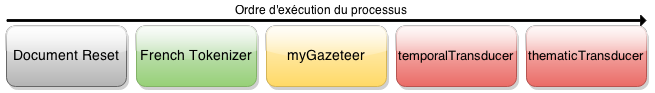
\includegraphics[scale=.5]{img/notreChaine.png}
\end{figure}
N'ayant besoin que de repérer les mots (Token) pour notre annotation, nous n'avons gardé que le Tokenizer. Ensuite, 
\begin{description}
\item[myGazeteer] contient les deux gazetiers que nous avons réalisés.
\item[temporalTransducer] contient les règles JAPE du domaine Temporel.
\item[thematicTransducer] contient les règles JAPE du domaine Thématique.
\end{description}
\part{Conclusion}
\section{Bilan du projet}
\begin{figure}[hbtp]
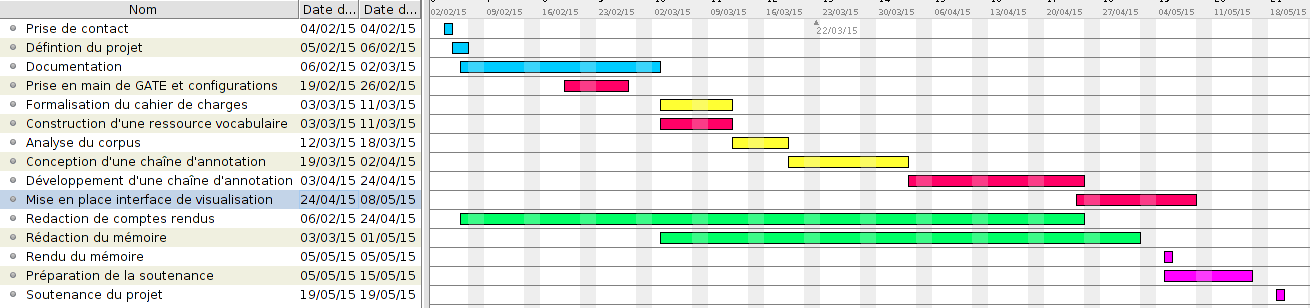
\includegraphics[scale=.3]{img/ganttEff.png}
\end{figure}
En comparant notre planning effectif au planning prévisionnel, il ressort que nous avons respecté le planning prévisionnel pour la première phase du projet et aussi toute la phase de rédaction des différents comptes rendus de réunion. La première phase comprenant la documentation, la prise en main des outils de travail, la formalisation du cahier de charge et l'étape de conception. Ce fut une phase de recherche pendant laquelle il nous est paru nécessaire de de bien cerner le domaine d'étude et aussi de mettre en place une bonne conception. Nous avions donc prévu pour cette phase une période de travail plus longue. En revanche, nous fut impossible de respecter le planning prévisionnel pour la phase de développement. En effet, notre chaîne de traitement est aboutie mais l'interface web de visualisation des résultats d'annotation quant à elle est toujours en cours de développement et sera présentée lors de la soutenance du projet.
\section{Expériences acquises}
Il est important de noter plusieurs retours d'expérience.\\D'abord la gestion du temps pour suivre convenablement un planning prévisionnel: nous retenons qu'il est assez improbable de respecter un planning prévisionnel, surtout pendant la phase de développement en raison du fait qu'on peut être confronté à des difficultés techniques (code) dans cette étape.\\
Ensuite la capacité de pouvoir fournir un produit final à un client qui respecte au mieux les spécifications exprimées dans un cahier de charges. On peut noter qu'il est primordial d'être fréquemment en contact avec le client pour mieux cerner et comprendre ses besoins. En effet, sur ce projet, le rôle de client fût joué par nos encadrants et celui du prestataire joué par nous.
Enfin, la préparation des réunions de travail qui passe par la rédaction d'ordres du jour et de comptes rendus, est une expérience supplémentaire que nous avons acquise.\\
Nous pensons que toutes ces expériences pourront nous être utiles à l'avenir dans le monde professionnel.
\newpage
\bibliography{latestbib}
\bibliographystyle{alpha}
\appendix
\chapter{Règles JAPE}
periode.jape
\includecode{code/temporelle/periode.jape}
periode\_emission.jape
\includecode{code/temporelle/periode_emission.jape}
legende.jape
\includecode{code/thematique/legende.jape}
nature\_monnaie.jape
\includecode{code/thematique/nature_monnaie.jape}
tresors.jape
\includecode{code/thematique/tresors.jape}
tresors\_details.jape
\includecode{code/thematique/tresors_details.jape}
trouvailles.jape
\includecode{code/thematique/trouvailles.jape}
trouvailles\_details.jape
\includecode{code/thematique/trouvailles_details.jape}
\end{document}
